\chapter{Project Architecture \& Choice Of Technologies}
\setcounter{minitocdepth}{1}
\minitoc
\newpage

\section{Introduction}
This chapter provides an overview of the project architecture and the choice of technologies used in the development process. It aims to explain the rationale behind the selection of specific architectural patterns, frameworks, and tools. By understanding the project architecture and the technologies employed, readers will gain insights into the design principles and the technical foundations of the system. Additionally, this chapter highlights the importance of making informed decisions when it comes to selecting technologies that align with the project requirements and objectives.

\section{Project Architecture - Modular Monolith}
The project architecture of Converty follows a Modular Monolith approach, which combines the benefits of a monolithic architecture with modular design principles. This section provides an in-depth look at the backend and services, frontend web dashboard, frontend mobile app, and the database used in the project.
The main architecture of Converty is shown in Figure \ref{fig:mainArchitecture}.

\begin{figure}[H]
    \centering
    \includegraphics[width=0.8\textwidth]{Images/mainArchitecture.png}
    \caption{Main Architecture}
    \label{fig:mainArchitecture}
\end{figure}

\subsection{Backend \& Services}
The backend of Converty, which follows a Modular Monolith architecture, is implemented using Node.js and Express.js. It encompasses the authentication system, simple CRUD operations, and the business logic. On the other hand, the microservices, developed in Go (Golang), handle specific tasks such as sending notifications, cron jobs, serverless functions, and other background tasks. This architectural approach ensures a flexible and scalable system capable of efficiently handling diverse workloads.

\subsubsection{Node.js - Express.js}
Node.js is a free, open-source, cross-platform JavaScript runtime environment that lets developers create servers, web apps, command line tools, and scripts \cite{nodejs}. It is built on the V8 JavaScript engine and provides a non-blocking, event-driven architecture that is ideal for building scalable network applications. Express.js is a minimal and flexible Node.js web application framework that provides a robust set of features for web and mobile applications \cite{expressjs}. It simplifies the process of building APIs and web applications by providing a robust set of features and middleware. Express.js is known for its simplicity, performance, and extensibility, making it an excellent choice for building the backend of the application.

\begin{figure}[H]
    \centering
    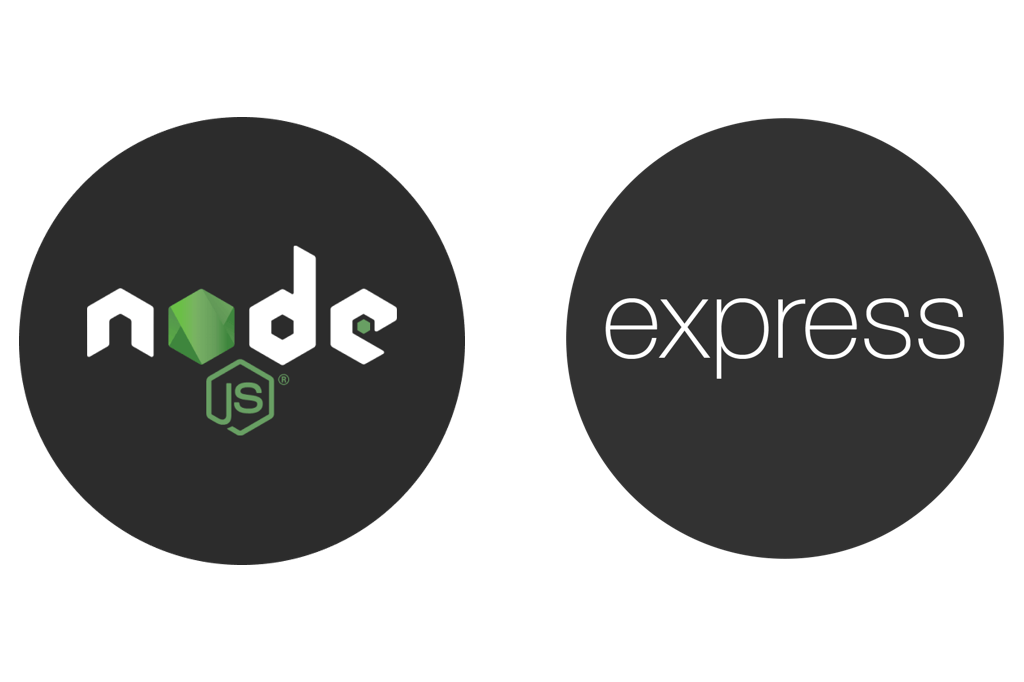
\includegraphics[width=0.5\textwidth]{Images/nodeAndExpress.png}
    \caption{Node.js and Express.js}
    \label{fig:nodeAndExpress}
\end{figure}

The benefits of using Node.js and Express.js for the backend of Converty include:

\begin{itemize}
    \item \textbf{Performance:} Node.js is known for its high performance due to its non-blocking, event-driven architecture. This allows the application to handle a large number of concurrent connections efficiently.
    \item \textbf{Scalability:} Node.js is designed to be scalable, making it suitable for applications that need to handle a large number of users and requests.
    \item \textbf{Simplicity:} Express.js provides a simple and intuitive API that makes it easy to build APIs and web applications.
    \item \textbf{Extensibility:} Express.js is highly extensible, allowing developers to add middleware and plugins to enhance the functionality of the application.
    \item \textbf{Community Support:} Node.js and Express.js have a large and active community that provides support, documentation, and a wide range of libraries and plugins.
    \item \textbf{Flexibility:} Node.js and Express.js are flexible and can be used to build a wide range of applications, from simple APIs to complex web applications.
    \item \textbf{Compatibility:} Node.js and Express.js are compatible with a wide range of databases, libraries, and tools, making it easy to integrate them with other technologies.
\end{itemize}

\subsubsection{Go (Golang)}
Go, also known as Golang, is an open-source, compiled, and statically typed programming language designed by Google. It is built to be simple, high-performing, readable, and efficient \cite{golang}. Go is known for its performance, simplicity, and ease of use, making it an excellent choice for building microservices. It is widely used in the industry for building high-performance applications, cloud services, and distributed systems. The microservices in Converty are developed in Go to handle specific tasks such as sending notifications, cron jobs, serverless functions, and other background tasks.

\begin{figure}[H]
    \centering
    
\includegraphics[width=0.5\textwidth]{Images/golang2.png}
    \caption{Go (Golang)}
    \label{fig:golang}
\end{figure}

The benefits of using Go for building microservices in Converty include:

\begin{itemize}
    \item \textbf{Performance:} Go is known for its high performance and efficiency, making it suitable for building high-performance applications.
    \item \textbf{Concurrency:} Go provides built-in support for concurrency, making it easy to write concurrent programs that can efficiently utilize multiple cores.
    \item \textbf{Simplicity:} Go has a simple and clean syntax that is easy to learn and use, making it ideal for building microservices.
    \item \textbf{Reliability:} Go is designed to be reliable and robust, with built-in error handling and garbage collection.
    \item \textbf{Scalability:} Go is designed to be scalable, making it suitable for building microservices that need to handle a large number of requests.
    \item \textbf{Community Support:} Go has a large and active community that provides support, documentation, and a wide range of libraries and tools.
    \item \textbf{Cross-Platform:} Go is cross-platform and can be compiled to run on different operating systems, making it easy to deploy microservices on different platforms.
\end{itemize}

\subsubsection{RabbitMQ}
RabbitMQ is a message-queueing software also known as a message broker or queue manager. Simply said, it is software where queues are defined, to which applications connect in order to transfer a message or messages \cite{rabbitmq}. RabbitMQ is used to implement asynchronous communication between microservices in Converty. It provides a reliable and scalable messaging system that allows microservices to communicate with each other in a decoupled and asynchronous manner. RabbitMQ supports multiple messaging protocols, including AMQP, MQTT, and STOMP, making it suitable for building distributed systems.

\begin{figure}[H]
    \centering
    
\includegraphics[width=0.2\textwidth]{Images/rabbitmq.png}
    \caption{RabbitMQ}
    \label{fig:rabbitmq}
\end{figure}

The benefits of using RabbitMQ for asynchronous communication between microservices in Converty include:

\begin{itemize}
    \item \textbf{Reliability:} RabbitMQ provides reliable message delivery and ensures that messages are not lost even in the event of failures.
    \item \textbf{Scalability:} RabbitMQ is designed to be scalable and can handle a large number of messages and connections.
    \item \textbf{Decoupling:} RabbitMQ allows microservices to communicate with each other in a decoupled manner, reducing dependencies between services.
    \item \textbf{Asynchronous Communication:} RabbitMQ supports asynchronous communication, allowing microservices to communicate with each other without blocking.
    \item \textbf{Multiple Protocols:} RabbitMQ supports multiple messaging protocols, making it suitable for building distributed systems that use different messaging protocols.
    \item \textbf{Monitoring:} RabbitMQ provides monitoring and management tools that allow developers to monitor the performance and health of the messaging system.
    \item \textbf{Community Support:} RabbitMQ has a large and active community that provides support, documentation, and a wide range of plugins and tools.
\end{itemize}

\subsection{Frontend - Web Dashboard}
The frontend of Converty, which is a web dashboard, is implemented using React, Vite, and TypeScript. React is a popular JavaScript library for building user interfaces, while Vite is a modern build tool that provides a fast and efficient development experience. TypeScript is a statically typed superset of JavaScript that adds type checking and other features to the language. The combination of React, Vite, and TypeScript provides a powerful and flexible frontend development environment that is ideal for building modern web applications.

\subsubsection{React + Vite + TypeScript}
Vite is a modern, fast build tool that provides an excellent development experience for modern web projects. Combining Vite with TypeScript and React allows developers to harness the power of fast builds, hot module replacement, and a highly efficient development workflow \cite{vite}. The four templates in Converty are also coded using React, Vite, and TypeScript. These templates provide the result online store that the shop owner configured. By using React, Vite, and TypeScript, the templates are able to leverage the benefits of these technologies, including component-based development, fast development and hot module replacement, and type safety. This ensures a consistent and efficient development process for creating and maintaining the shop owners' online shop.

\begin{figure}[H]
    \centering
    
\includegraphics[width=0.5\textwidth]{Images/reactViteTs.png}
    \caption{React + Vite + TypeScript}
    \label{fig:reactViteTypeScript}
\end{figure}

The benefits of using React, Vite, and TypeScript for the frontend of Converty include:

\begin{itemize}
    \item \textbf{Component-Based Development:} React allows developers to build reusable and composable components that can be easily shared and reused across the application.
    \item \textbf{Fast Development:} Vite provides fast development and hot module replacement, allowing developers to see changes in real-time without reloading the page.
    \item \textbf{Type Safety:} TypeScript adds type checking and other features to JavaScript, making it easier to catch errors and write more reliable code.
    \item \textbf{Performance:} React and Vite are known for their performance and efficiency, making them suitable for building fast and responsive web applications.
    \item \textbf{Community Support:} React, Vite, and TypeScript have large and active communities that provide support, documentation, and a wide range of libraries and tools.
    \item \textbf{Flexibility:} React, Vite, and TypeScript are flexible and can be used to build a wide range of web applications, from simple websites to complex web applications.
    \item \textbf{Scalability:} React, Vite, and TypeScript are designed to be scalable, making them suitable for building web applications that need to handle a large number of users and requests.
\end{itemize}

\subsubsection{Redux}
Redux is a predictable state container for JavaScript applications that helps manage the state of the application in a consistent and predictable way. It provides a single source of truth for the state of the application and allows changes to the state to be made in a predictable and controlled manner. Redux is used in the frontend of Converty to manage the state of the application, including user authentication, data fetching, and UI state.

\begin{figure}[H]
    \centering
    
\includegraphics[width=0.2\textwidth]{Images/redux.png}
    \caption{Redux}
    \label{fig:redux}
\end{figure}

The benefits of using Redux for state management in the frontend of Converty include:

\begin{itemize}
    \item \textbf{Predictability:} Redux provides a predictable state container that helps manage the state of the application in a consistent and predictable way.
    \item \textbf{Single Source of Truth:} Redux provides a single source of truth for the state of the application, making it easier to manage and update the state.
    \item \textbf{Debugging:} Redux provides tools for debugging and monitoring the state of the application, making it easier to identify and fix issues.
    \item \textbf{Scalability:} Redux is designed to be scalable, making it suitable for building large and complex web applications.
    \item \textbf{Community Support:} Redux has a large and active community that provides support, documentation, and a wide range of plugins and tools.
    \item \textbf{Middleware:} Redux provides middleware that allows developers to add custom logic and side effects to the state management process.
    \item \textbf{Performance:} Redux is known for its performance and efficiency, making it suitable for building fast and responsive web applications.
\end{itemize}

\subsection{Frontend - Mobile App}

\subsubsection{React Native}
React Native is an open-source UI software framework created by Facebook Inc. (now Meta Platforms). It is used to develop applications for Android, Android TV, iOS, macOS, tvOS, Web, Windows, and UWP by enabling developers to use the React framework along with native platform capabilities \cite{reactnative}. It is used to develop Android and iOS applications at Facebook, Microsoft, and Shopify. It is also being used to develop virtual reality applications at Oculus. The mobile app of Converty is implemented using React Native, a popular framework for building cross-platform mobile applications. React Native allows developers to build mobile apps using JavaScript and React, providing a fast and efficient development experience. By using React Native, Converty is able to build a mobile app that runs on both iOS and Android devices, reducing development time and cost.

\begin{figure}[H]
    \centering
    
\includegraphics[width=0.3\textwidth]{Images/reactNative.png}
    \caption{React Native}
    \label{fig:reactNative}
\end{figure}

The benefits of using React Native for building the mobile app of Converty include:

\begin{itemize}
    \item \textbf{Cross-Platform:} React Native allows developers to build mobile apps that run on both iOS and Android devices, reducing development time and cost.
    \item \textbf{Efficiency:} React Native provides a fast and efficient development experience, allowing developers to build mobile apps quickly and easily.
    \item \textbf{Performance:} React Native is known for its performance and efficiency, making it suitable for building fast and responsive mobile apps.
    \item \textbf{Community Support:} React Native has a large and active community that provides support, documentation, and a wide range of libraries and tools.
    \item \textbf{Hot Reloading:} React Native provides hot reloading, allowing developers to see changes in real-time without reloading the app.
    \item \textbf{Native Components:} React Native provides access to native components and APIs, allowing developers to build mobile apps with a native look and feel.
    \item \textbf{Code Reusability:} React Native allows developers to reuse code across different platforms, reducing duplication and improving maintainability.
\end{itemize}

\subsubsection{Expo}
Expo is an open-source platform for making universal native apps that run on Android, iOS, and the web. It includes a universal runtime and libraries that let you build native apps by writing React and JavaScript \cite{expo}. Expo is a set of tools and services that help developers build React Native applications more easily. It provides a fast and efficient development environment, allowing developers to build, test, and deploy mobile apps quickly. Expo provides a wide range of features and APIs, including push notifications, camera access, and location services, making it easy to build feature-rich mobile apps.

\begin{figure}[H]
    \centering
    
\includegraphics[width=0.2\textwidth]{Images/expo.png}
    \caption{Expo}
    \label{fig:expo}
\end{figure}

The benefits of using Expo for building the mobile app of Converty include:

\begin{itemize}
    \item \textbf{Fast Development:} Expo provides a fast and efficient development environment, allowing developers to build mobile apps quickly and easily.
    \item \textbf{Feature-Rich:} Expo provides a wide range of features and APIs, including push notifications, camera access, and location services, making it easy to build feature-rich mobile apps.
    \item \textbf{Community Support:} Expo has a large and active community that provides support, documentation, and a wide range of libraries and tools.
    \item \textbf{Cross-Platform:} Expo allows developers to build mobile apps that run on both iOS and Android devices, reducing development time and cost.
    \item \textbf{Hot Reloading:} Expo provides hot reloading, allowing developers to see changes in real-time without reloading the app.
    \item \textbf{Ease of Use:} Expo is easy to use and provides a simple and intuitive API that makes it easy to build mobile apps.
    \item \textbf{Performance:} Expo is known for its performance and efficiency, making it suitable for building fast and responsive mobile apps.
\end{itemize}

\subsubsection{Zustand}
Zustand is a small, fast, and scalable bearbones state management solution. Zustand has a comfy API based on hooks. It isn't boilerplatey or opinionated, but has enough convention to be explicit and flux-like \cite{zustand}. Zustand is a simple and fast state management library for React applications. It provides a way to manage the state of the application in a simple and efficient way, reducing the complexity of managing state in React components. Zustand is used in the mobile app of Converty to manage the state of the application, including user authentication, data fetching, and UI state.

\begin{figure}[H]
    \centering
    
\includegraphics[width=0.2\textwidth]{Images/zustand.png}
    \caption{Zustand}
    \label{fig:zustand}
\end{figure}

The benefits of using Zustand for state management in the mobile app of Converty include:

\begin{itemize}
    \item \textbf{Simplicity:} Zustand provides a simple and intuitive API that makes it easy to manage the state of the application.
    \item \textbf{Performance:} Zustand is known for its performance and efficiency, making it suitable for building fast and responsive mobile apps.
    \item \textbf{Predictability:} Zustand provides a predictable state container that helps manage the state of the application in a consistent and predictable way.
    \item \textbf{Community Support:} Zustand has a large and active community that provides support, documentation, and a wide range of plugins and tools.
    \item \textbf{Flexibility:} Zustand is flexible and can be used to manage the state of the application in a wide range of scenarios.
    \item \textbf{Scalability:} Zustand is designed to be scalable, making it suitable for building large and complex mobile apps.
    \item \textbf{Performance:} Zustand is known for its performance and efficiency, making it suitable for building fast and responsive mobile apps.
\end{itemize}

\subsection{Database - MongoDB}
MongoDB is a document database with the scalability and flexibility that you want with the querying and indexing that you need \cite{mongodb}. MongoDB is a popular NoSQL database that is used in Converty to store data such as user information, product information, and configuration data. MongoDB is a document-oriented database that provides a flexible and scalable data storage solution. It is known for its performance, scalability, and ease of use, making it an excellent choice for building modern web applications.

\begin{figure}[H]
    \centering
    
\includegraphics[width=0.2\textwidth]{Images/mongodb2.png}
    \caption{MongoDB}
    \label{fig:mongodb}
\end{figure}

The benefits of using MongoDB for storing data in Converty include:

\begin{itemize}
    \item \textbf{Flexibility:} MongoDB is a document-oriented database that provides a flexible data storage solution, allowing developers to store data in a schema-less format.
    \item \textbf{Scalability:} MongoDB is designed to be scalable, making it suitable for building web applications that need to handle a large amount of data.
    \item \textbf{Performance:} MongoDB is known for its performance and efficiency, making it suitable for building fast and responsive web applications.
    \item \textbf{Ease of Use:} MongoDB is easy to use and provides a simple and intuitive API that makes it easy to interact with the database.
    \item \textbf{Community Support:} MongoDB has a large and active community that provides support, documentation, and a wide range of tools and libraries.
    \item \textbf{Compatibility:} MongoDB is compatible with a wide range of programming languages, frameworks, and tools, making it easy to integrate with other technologies.
\end{itemize}

\subsubsection{Data Modeling - Mongoose}
Mongoose is an Object Data Modeling (ODM) library for MongoDB and Node.js. It manages relationships between data, provides schema validation, and is used to translate between objects in code and the representation of those objects in MongoDB \cite{mongoose}. Mongoose provides a schema-based solution for modeling data, allowing developers to define the structure of the data and enforce validation rules. Mongoose is used in Converty to model data in MongoDB, including user information, product information, and configuration data.

The benefits of using Mongoose for data modeling in Converty include:

\begin{itemize}
    \item \textbf{Schema-Based:} Mongoose provides a schema-based solution for modeling data in MongoDB, allowing developers to define the structure of the data and enforce validation rules.
    \item \textbf{Validation:} Mongoose provides built-in validation features that allow developers to enforce validation rules on the data.
    \item \textbf{Relationships:} Mongoose provides support for defining relationships between different types of data, making it easy to model complex data structures.
    \item \textbf{Middleware:} Mongoose provides middleware that allows developers to add custom logic and side effects to the data modeling process.
    \item \textbf{Community Support:} Mongoose has a large and active community that provides support, documentation, and a wide range of plugins and tools.
    \item \textbf{Performance:} Mongoose is known for its performance and efficiency, making it suitable for modeling data in MongoDB.
    \item \textbf{Scalability:} Mongoose is designed to be scalable, making it suitable for modeling large and complex data structures.
\end{itemize}

\subsubsection{Caching - Redis}
Redis is the world’s fastest in-memory database. It provides cloud and on-prem solutions for caching, vector search, and NoSQL databases that seamlessly fit into any tech stack—making it simple for digital customers to build, scale, and deploy the fast apps our world runs on \cite{redis}. Redis is used in Converty for caching data such as user sessions, product information, and configuration data. Redis provides a fast and efficient way to store and retrieve data in memory, making it ideal for caching frequently accessed data. It is known for its performance, scalability, and reliability, making it an excellent choice for building modern web applications.

\begin{figure}[H]
    \centering
    
\includegraphics[width=0.2\textwidth]{Images/redis.png}
    \caption{Redis}
    \label{fig:redis}
\end{figure}

The benefits of using Redis for caching data in Converty include:

\begin{itemize}
    \item \textbf{Performance:} Redis is an in-memory data store that provides fast and efficient data storage and retrieval.
    \item \textbf{Scalability:} Redis is designed to be scalable, making it suitable for caching large amounts of data.
    \item \textbf{Reliability:} Redis is known for its reliability and fault tolerance, making it suitable for building high-availability applications.
    \item \textbf{Ease of Use:} Redis is easy to use and provides a simple and intuitive API that makes it easy to interact with the data store.
    \item \textbf{Community Support:} Redis has a large and active community that provides support, documentation, and a wide range of tools and libraries.
    \item \textbf{Performance:} Redis is known for its performance and efficiency, making it suitable for caching data in modern web applications.
    \item \textbf{Scalability:} Redis is designed to be scalable, making it suitable for caching large amounts of data in memory.
\end{itemize}

\section{Conclusion}

In conclusion, the project architecture of Converty is designed to be modular, scalable, and efficient. By using a combination of Node.js, Express.js, Go, React, Vite, TypeScript, Redux, React Native, Expo, MongoDB, Mongoose, RabbitMQ, and Redis, Converty is able to build a flexible and feature-rich system that meets the requirements of modern web applications. The choice of technologies is based on their performance, scalability, reliability, ease of use, and community support. By selecting the right technologies and architectural patterns, Converty is able to build a robust and reliable system that can handle diverse workloads and provide a seamless user experience.